\documentclass{article}
\usepackage[utf8]{inputenc}
\usepackage[includeheadfoot, margin=1em,headheight=2em]{geometry}
\usepackage{titling}
\geometry{a4paper, left=2cm, right=2cm, top=2cm, bottom=2cm}
\usepackage{graphicx}
\usepackage{float}
\providecommand{\versionnumber}{1.0.0}
\usepackage{enumitem}
\usepackage{array}
\usepackage[italian]{babel}
\newcolumntype{P}[1]{>{\centering\arraybackslash}p{#1}}
\renewcommand{\arraystretch}{1.5} % Default value: 1
\setlength{\droptitle}{-6em}

%font
\usepackage[defaultfam,tabular,lining]{montserrat}
\usepackage[T1]{fontenc}
\renewcommand*\oldstylenums[1]{{\fontfamily{Montserrat-TOsF}\selectfont #1}}

%custom bold 
\usepackage[outline]{contour}
\usepackage{xcolor}
\newcommand{\custombold}{\contour{black}}

%table colors
\usepackage{color, colortbl}
\definecolor{Blue}{rgb}{0.51,0.68,0.79}
\definecolor{LightBlue}{rgb}{0.82,0.87,0.90}
\definecolor{LighterBlue}{rgb}{0.93,0.95,0.96}

%Header
\usepackage{fancyhdr, xcolor}
\pagestyle{fancy}
\let\oldheadrule\headrule% Copy \headrule into \oldheadrule
\renewcommand{\headrule}{\color{Blue}\oldheadrule}% Add colour to \headrule
\renewcommand{\headrulewidth}{0.2em}
\fancyhead[L]{Studio IBM Process Mining}
\fancyhead[C]{Samuele Vignotto}
\fancyhead[R]{
\includegraphics[height=1cm]{Logo/Y_LOGO-SOLO.png}}
\setcounter{secnumdepth}{0}

\title{\Huge{\textbf{IBM Process Mining}}\vspace{-1em}}
\author{Samuele Vignotto}
\date{}
\begin{document}
\maketitle
\begin{figure}[h]
  \centering
  
\includegraphics[width=6cm, height=6cm]{Logo/Y_LOGO-SOLO.png}
  \label{fig:immagine}
\end{figure}

\newpage
\tableofcontents
\newpage

\section{Introduzione}

IBM Process Mining è uno strumento per l'analisi e l'ottimizzazione dei processi aziendali, progettato per fornire una comprensione di come i processi vengono realmente eseguiti all'interno di un'organizzazione. Grazie alla capacità di sfruttare i dati storici raccolti da diverse fonti aziendali, IBM Process Mining permette di ricostruire il flusso di lavoro effettivo, individuando inefficienze e deviazioni rispetto ai processi ideali.\\
La visualizzazione dettagliata dei processi è uno degli aspetti chiave della soluzione, consentendo agli utenti di vedere come le attività si susseguono nel tempo. Inoltre, lo strumento identifica automaticamente i colli di bottiglia e le ridondanze.\\
Un'altra funzione essenziale di IBM Process Mining è la sua integrazione con tecnologie di automazione e intelligenza artificiale. Questo permette di creare flussi di lavoro automatizzati che semplificano le attività ripetitive, riducendo l'intervento manuale e minimizzando il rischio di errori. Inoltre, lo strumento supporta un monitoraggio continuo delle prestazioni dei processi, consentendo una gestione proattiva e miglioramenti progressivi in tempo reale.\\
Le funzionalità di simulazione offerte da IBM Process Mining permettono di testare vari scenari e prevedere l’impatto di eventuali modifiche, facilitando così un processo decisionale informato e basato sui dati. L’integrazione con altre soluzioni IBM, come Watson AI e IBM Cloud, fornisce ulteriori opportunità di ottimizzazione e di trasformazione digitale su larga scala.

\section{Formati di file accettati}
IBM Process Mining supporta diversi formati di file per l'importazione e l'esportazione dei dati, permettendo la flessibilità nell'integrazione con altri strumenti e l'analisi dei processi.

\subsection{CSV (Comma-Separated Values)}
Utilizzato per l'importazione e l'esportazione di dati di origine. È il formato principale per caricare dati da sistemi aziendali e fonti esterne.

\subsection{BPMN 2.0 (Business Process Model and Notation)}
Formato utilizzato per esportare modelli di processo in un linguaggio standard per la modellazione dei processi aziendali. Supporta formati specifici come Bizagi, Bonita, Camunda e IBM Blueworks.

\subsection{XPDL (XML Process Definition Language) 2.1}
Permette di esportare i processi in un formato XML utilizzato comunemente per la definizione di workflow.

\subsection{XES (eXtensible Event Stream)}
Un formato di file standardizzato per rappresentare i log di eventi di processo, utilizzato principalmente per l'analisi dei processi con strumenti di process mining.

\subsection{SVG (Scalable Vector Graphics)}
Utilizzato per l'esportazione di modelli di processo in formato immagine vettoriale, utile per visualizzazioni grafiche di alta qualità dei processi.

\section{Funzionalità}

\subsection{Scoperta dei processi}
IBM Process Mining è in grado di analizzare i log degli eventi provenienti dai sistemi aziendali per generare modelli di processo end-to-end. Questo permette di visualizzare come i processi vengono effettivamente eseguiti, incluse tutte le attività e i percorsi processuali coinvolti.

\subsection{Analisi delle performance}
Lo strumento offre funzionalità per monitorare e valutare la performance dei processi. Questo include l'analisi dei tempi di ciclo, i costi associati a ogni fase del processo, le deviazioni rispetto ai modelli di riferimento e i colli di bottiglia che causano inefficienze operative.

\subsection{Conformance checking}
IBM Process Mining consente di verificare la conformità dei processi rispetto ai modelli di riferimento. Attraverso il confronto dei processi scoperti con i processi teorici o standard, è possibile individuare le deviazioni e correggere le inefficienze.

\subsection{Simulazione dei processi}
La funzionalità di simulazione consente di creare e testare scenari "what-if", simulando modifiche al flusso di lavoro e prevedendo l'impatto di tali modifiche su tempi, costi e risorse. Questa capacità è fondamentale per supportare il processo decisionale in un ambiente basato sui dati.

\subsection{Automazione dei processi}
IBM Process Mining facilita l'automazione dei processi attraverso l'integrazione con strumenti di automazione e RPA (Robotic Process Automation). Identifica i migliori candidati per l'automazione, stima i benefici in termini di costi e performance e genera automaticamente script RPA per automatizzare le attività ripetitive e manuali.

\subsection{Monitoraggio continuo}
È possibile configurare monitoraggi personalizzati per i KPI dei processi, impostare soglie e intervalli di monitoraggio e ricevere notifiche automatiche in caso di anomalie. Questo consente una gestione proattiva dei processi, prevenendo criticità e garantendo il miglioramento continuo.

\subsection{Personalizzazione e dashboard}
IBM Process Mining fornisce dashboard configurabili e interattive che consentono di visualizzare i dati di processo in modo personalizzato. Gli utenti possono filtrare, ordinare e rappresentare i dati per ottenere le informazioni più rilevanti per la loro organizzazione, supportando così l'analisi decisionale.

\section{Implementazioni pratiche: simulazioni}
Il file CSV è stato creato mediante uno script Python che simula una serie di attività relative alla produzione e alla gestione degli ordini di prodotti. Inoltre, per la simulazione dei dati, sono stati presi in considerazione anche i dati estratti manualmente da un database di un sistema gestionale.
\subsection{Regole di simulazione}
\subsubsection{Impostazione delle date iniziali}
Ogni ciclo di attività inizia con la prima attività programmata tra il 1 gennaio 2019 e il 31 dicembre 2020.\\
\subsubsection{Definizione delle tipologie di prodotti}
Viene creata una lista di 30 tipi di scarpe, denominate "Scarpe tipo 1" fino a "Scarpe tipo 30".\\
\subsubsection{Definizione delle attività e delle durate}
Sono state definite 17 attività, ciascuna con un ID unico e una durata variabile. Le durate delle attività sono espresse in minuti o giorni, a seconda dell'attività specifica.\\
\subsubsection{Generazione di un ciclo di attività per prodotto}
Per ciascun prodotto, viene generato un ciclo di attività che segue le seguenti regole:
\begin{itemize}
    \item \custombold{attività obbligatorie}: alcune attività avvengono in un ordine fisso. Ad esempio, "Conferma ordine" è sempre seguita da "Creazione progetto";
    \item \custombold{modifica del progetto}: un numero casuale di modifiche al progetto (da 1 a 5) può essere aggiunto dopo la creazione del progetto;
    \item \custombold{gestione degli ordini fornitore}: un numero casuale (da 1 a 3) di cicli di gestione ordini fornitore può essere inserito, ognuno dei quali può includere attività come "Ordine fornitore", "Arrivo offerta fornitore", "Ordine annullato" o "Ordine sospeso";
    \item \custombold{produzione}: vengono aggiunte attività relative alla produzione, come "Stampa scheda di produzione", "Inizio ciclo di produzione" e "Termine ordine di produzione";
    \item \custombold{attività non necessarie}: possono essere inserite attività opzionali come "Controllo qualità non necessario" (20\% di probabilità) e "Ri-lavorazione non necessaria" (10\% di probabilità);
    \item \custombold{consegna}: dopo la produzione, viene aggiunta l'attività di "Consegna".
\end{itemize}
\subsubsection{Generazione dei timestamp}
Ogni attività riceve un timestamp generato casualmente basato su un intervallo di tempo definito per quella specifica attività.
\subsubsection{Ciclo di generazione dei dati}
Il numero di prodotti varia tra 300 e 500, determinato casualmente. Per ogni prodotto, viene generato un ciclo di attività completo, assicurandosi che tutte le attività obbligatorie siano inserite nel corretto ordine e che le attività casuali siano distribuite come specificato.\\
\subsubsection{Mischiamento casuale delle righe del file CSV}
È stato utilizzato un algoritmo per mischiare in modo casuale le righe del file CSV. L'algoritmo legge il file CSV originale e separa l'intestazione dai dati. Successivamente, le righe dei dati vengono mescolate casualmente mantenendo intatta l'intestazione. Infine, il nuovo file CSV, con le righe mescolate, viene salvato in un file di output. Questo processo assicura che i dati siano riorganizzati in modo casuale senza alterare la struttura del file CSV.

\subsection{Modello}
\begin{figure}[H]
    \centering
    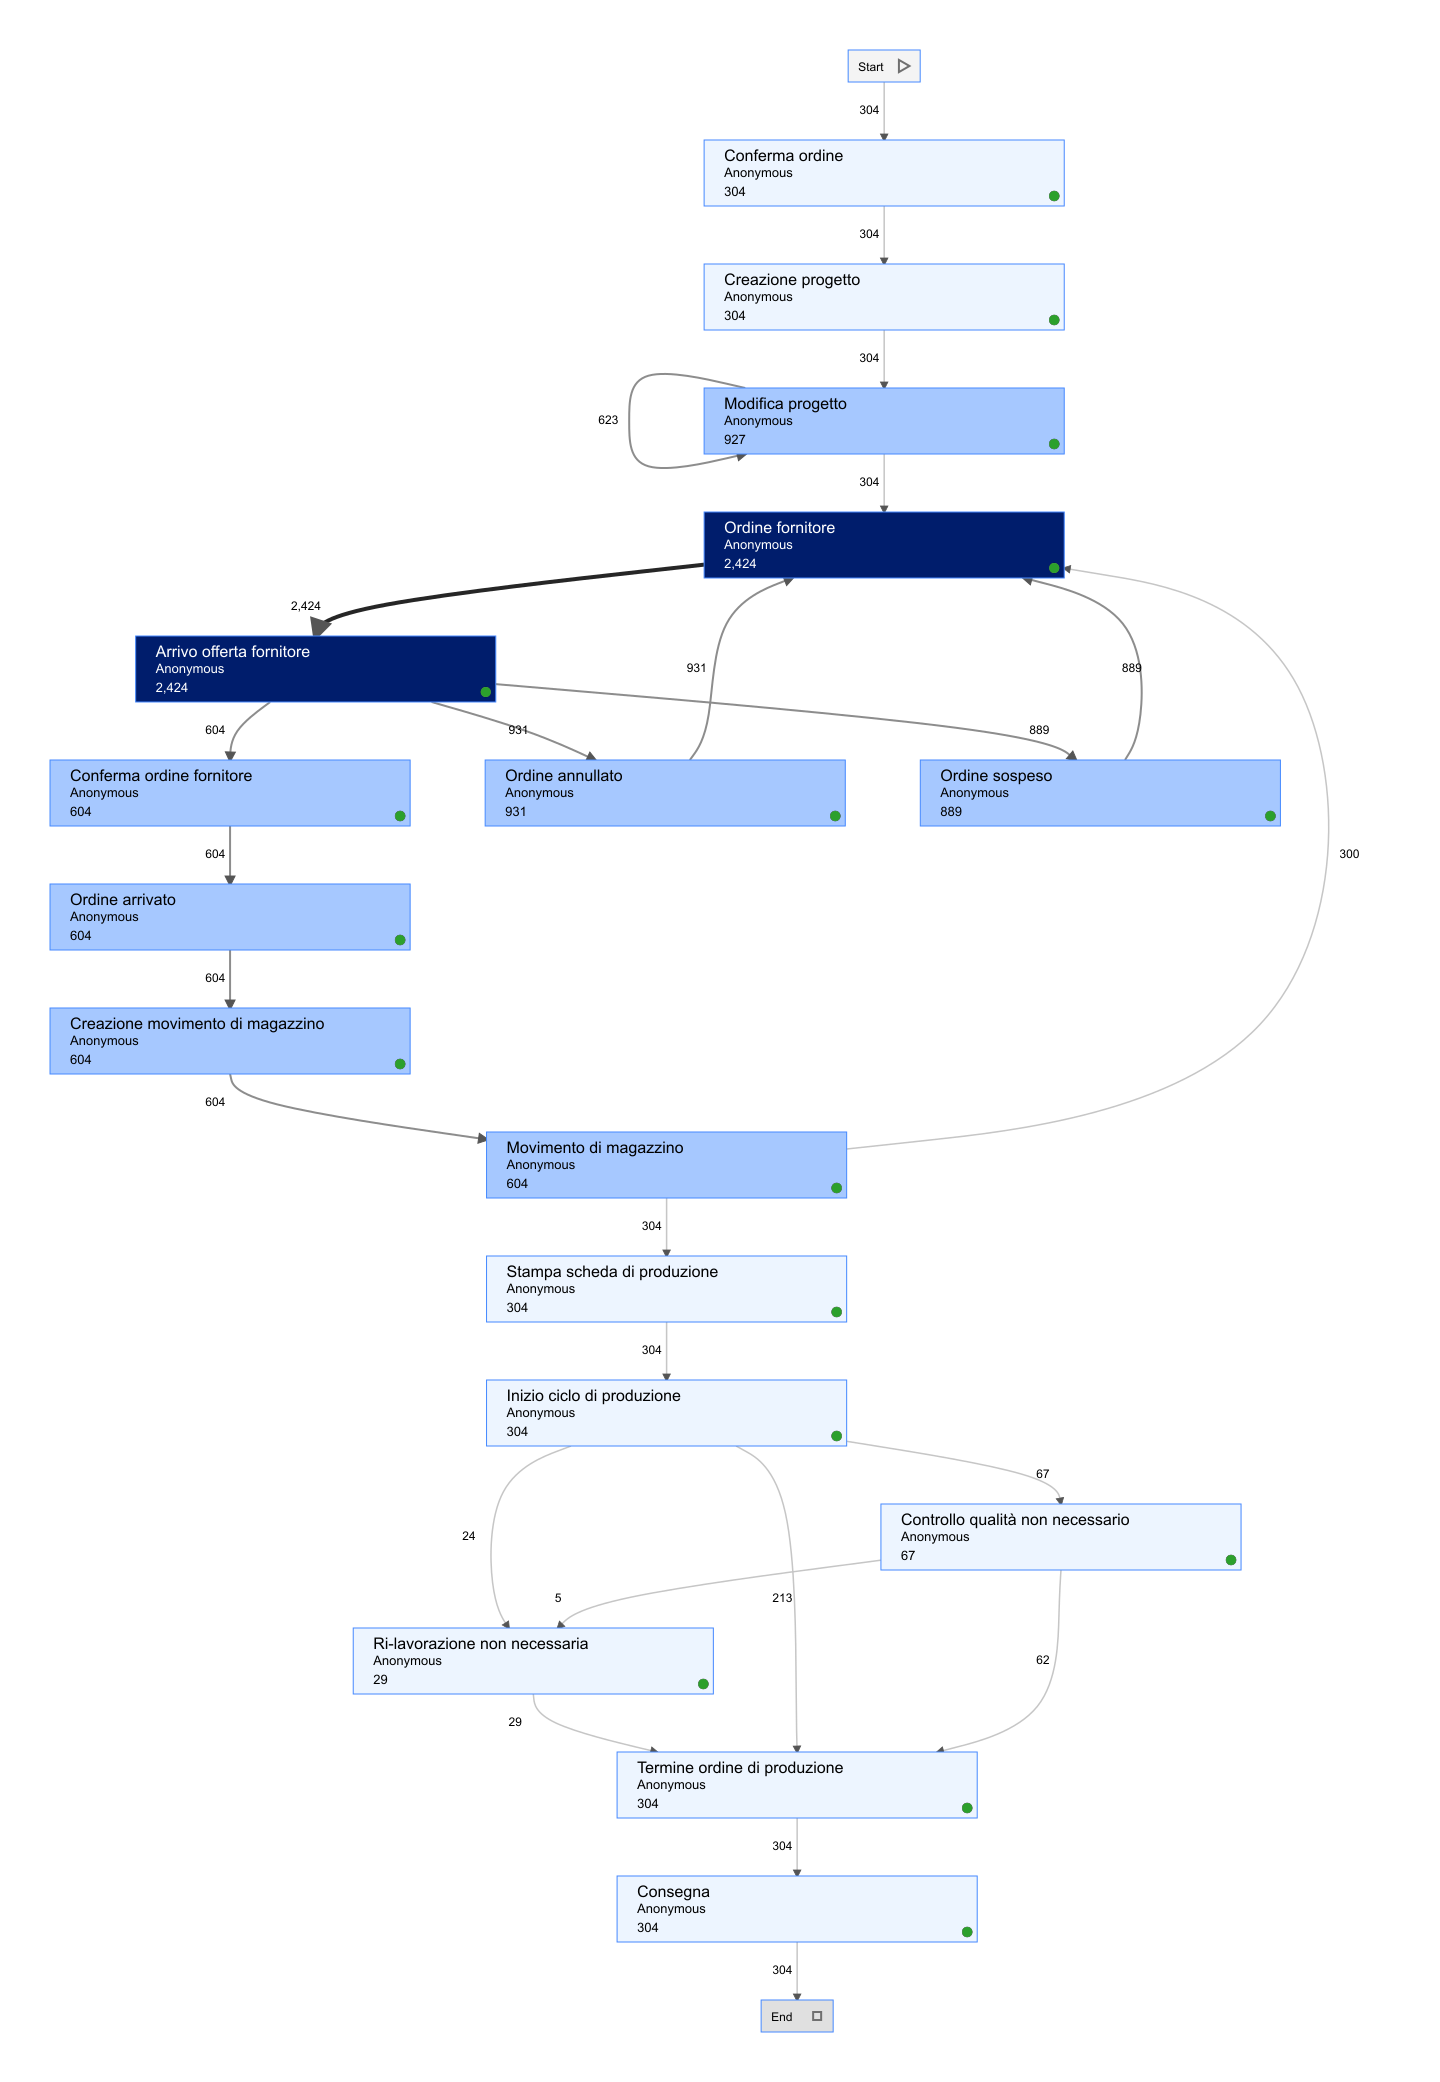
\includegraphics[width=\textwidth]{imgIBM/Simulazione/ModelloSimulazione.png}
    \caption{Modello del processo}
    \label{fig:process-model}
\end{figure}
La mappa di processo fornita rappresenta in modo chiaro e dettagliato i vari passaggi del flusso di lavoro e le possibili transizioni tra le attività. Ogni nodo rappresenta una fase specifica del processo, mentre le linee di collegamento mostrano le diverse direzioni che il flusso può prendere a seconda delle condizioni in cui si trova.\\
Un esempio rilevante è il passaggio tra "Ordine fornitore" e "Arrivo offerta fornitore". Questo segmento rappresenta un punto critico e frequente, che sottolinea l'importanza della relazione con i fornitori nel contesto produttivo. Al contrario, i percorsi verso "Ordine annullato" o "Ordine sospeso" sono meno comuni, segnalando che le cancellazioni o sospensioni non sono eventi ricorrenti, ma sono comunque contemplati come eccezioni gestibili.\\
La mappa offre quindi spunti significativi per miglioramenti. Le transizioni meno frequenti, come quelle che portano all'annullamento o sospensione, potrebbero rappresentare punti deboli del sistema o varianti che, sebbene rare, richiedono ulteriore attenzione e ottimizzazione per garantire una risposta efficiente in caso di imprevisti.\\
La struttura del flusso è coerente e riflette una chiara organizzazione temporale tra le attività, assicurando che ogni fase avvenga in sequenza logica.\\
 Le varianti di processo sono ben rappresentate e facilmente identificabili, permettendo di evidenziare i punti di forza, come la gestione rapida degli ordini e l'efficienza dei movimenti di magazzino, ma anche le aree che potrebbero richiedere ulteriore approfondimento, come la gestione degli ordini sospesi.

 \subsection{BPMN}
 \begin{figure}[H]
    \centering
    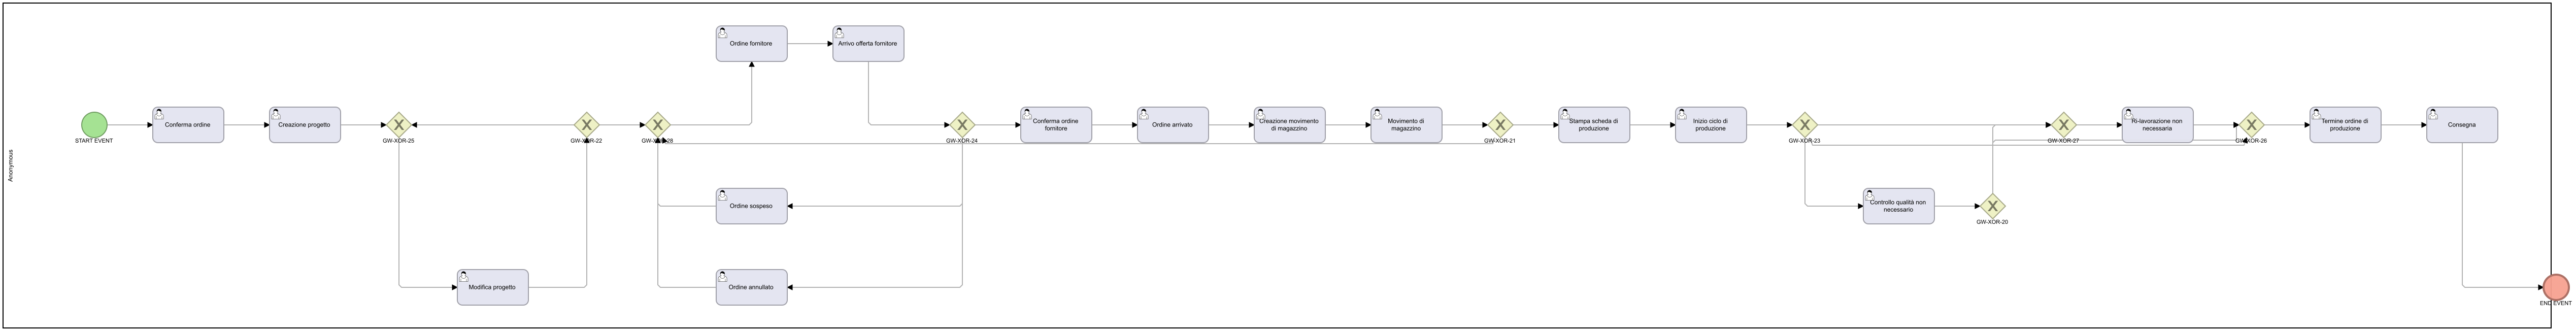
\includegraphics[width=\textwidth]{imgIBM/Simulazione/BPMNSimulazione.png}
    \caption{BPMN del processo}
    \label{fig:process-BPMN}
\end{figure}
Il modello BPMN qui presentato segue una struttura lineare che si sviluppa da sinistra verso destra, con attività sequenziali intervallate da gateway decisionali. Questo rende la mappa di facile lettura e interpretazione, poiché mantiene un flusso costante in cui le decisioni chiave sono ben delineate. I gateway di decisione sono chiaramente rappresentati da rombi, una convenzione standard in BPMN che facilita l'identificazione dei punti in cui il flusso può deviare in base a condizioni specifiche.\\
La separazione tra attività operative e decisioni è ben rispettata, mantenendo una distinzione visiva netta tra le azioni dirette, come "Conferma ordine" o "Movimento di magazzino", e le decisioni critiche del processo, come "Modifica progetto" o "Conferma ordine fornitore". Questo rafforza la comprensibilità del diagramma e aiuta gli utenti a identificare facilmente i passaggi chiave senza ambiguità.\\
Il modello presenta una logica sequenziale ben delineata, dove ogni attività si collega chiaramente alla successiva. L'uso di frecce per connettere le attività assicura che non ci siano ambiguità sul percorso che il flusso deve seguire. Tuttavia, il modello non fa emergere chiaramente eventuali parallelismi o sovrapposizioni temporali, aspetto che potrebbe essere utile per rappresentare attività che possono avvenire contemporaneamente.\\
Un altro aspetto è che, sebbene i gateway permettano la gestione di decisioni complesse, non è altrettanto evidente quale sia l'effettivo impatto temporale di ogni decisione sul processo.\\
Uno dei punti di forza principali di questo modello BPMN è la sua chiarezza. Le attività sono ben distribuite, con una separazione logica tra le fasi e un utilizzo efficace di gateway decisionali che mantengono il flusso ordinato. Tuttavia, la complessità introdotta dai numerosi rami decisionali potrebbe risultare eccessiva per utenti che cercano una rappresentazione ad alto livello o desiderano una vista più semplificata. In questo caso, l'uso di sottoprocessi o una rappresentazione gerarchica potrebbe aiutare a gestire meglio i dettagli senza compromettere la comprensione generale.\\
Un'altra possibile area di miglioramento riguarda la rappresentazione delle attività parallele e delle tempistiche. Attualmente, il modello non offre un’indicazione chiara di quali attività possano avvenire simultaneamente o di quanto tempo richiedano le varie fasi, informazioni che potrebbero essere utili in un'analisi più approfondita del processo.

\subsection{Statistiche}
\subsubsection{Panoramica del processo}
 \begin{figure}[H]
    \centering
    
\includegraphics[width=\textwidth]{imgIBM/Simulazione/PanoramicaProcessoSimulazione.png}
    \caption{Panoramica del processo}
    \label{fig:process-overview}
\end{figure}
Nel pannello "Prestazioni", viene indicato che il processo ha trattato un totale di 304 casi. Questo dato fornisce un'indicazione della mole complessiva di lavoro gestito dal sistema. Il "Tasso di arrivo", pari a 1,23 casi/giorno, rappresenta la frequenza con cui nuovi casi entrano nel sistema, il che suggerisce un flusso costante ma moderato di nuove istanze di processo.\\
Questa metrica del tasso di arrivo è utile per comprendere il carico quotidiano e può essere confrontata con la capacità operativa del sistema per determinare se ci sono sovraccarichi o, al contrario, margini per aumentare l'efficienza.\\
La parte centrale della panoramica riguarda i tempi di risposta, ovvero il tempo necessario per completare ogni caso dal momento in cui viene avviato fino alla sua conclusione. Viene fornito il tempo medio di risposta, pari a 39 giorni e 9 ore, che rappresenta il tempo medio richiesto per portare a termine un caso.\\

\subsubsection{Panoramica critica}
 \begin{figure}[H]
    \centering
    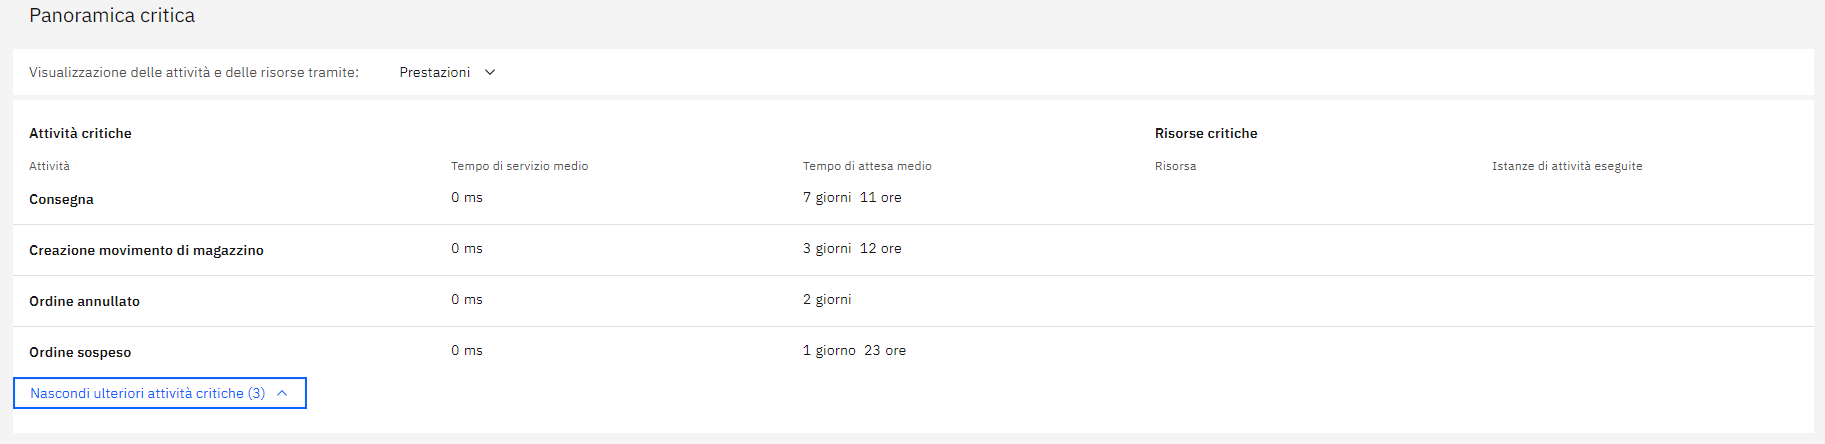
\includegraphics[width=\textwidth]{imgIBM/Simulazione/PanoramicaCriticaSimulazione.png}
    \caption{Panoramica delle attività critiche del processo}
    \label{fig:process-critical-activities-overview}
\end{figure}
Questa funzione serve a individuare quelle che vengono definite "attività critiche", ovvero fasi del processo che possono accumulare ritardi o che, pur avendo un impatto significativo, mostrano un'efficienza ridotta a causa di tempistiche di attesa o problematiche legate alle risorse. Non si tratta solo di un'analisi quantitativa, ma di una visione qualitativa che mira a migliorare le performance generali del processo.\\
Il valore principale di questa funzionalità sta nella sua capacità di dare agli utenti un'istantanea delle parti più vulnerabili del sistema senza dover navigare nell'intero processo o esaminare ciascuna attività nel dettaglio. Questa sintesi permette di concentrarsi su pochi elementi fondamentali e consente ai decisori aziendali o agli analisti di priorizzare gli interventi in modo informato.\\
La tabella è organizzata in modo semplice e intuitivo, con le attività critiche evidenziate in modo chiaro, ciascuna accompagnata da metriche fondamentali come il tempo di attesa medio e il tempo di servizio medio. La distinzione tra questi due valori è utile per separare i problemi legati all'efficienza operativa da quelli derivanti da colli di bottiglia o attese prolungate. L’inclusione delle risorse critiche, anche se non sempre valorizzata in questo esempio specifico, aggiunge un ulteriore livello di analisi, suggerendo dove la carenza o l'inefficienza delle risorse potrebbe rallentare il flusso.\\
La chiarezza e l'usabilità della funzione consentono decisioni rapide ed efficaci, con un focus mirato su come migliorare le parti più critiche del flusso di lavoro. Tuttavia non è inclusa una correlazione più diretta tra risorse e attività critiche.

\subsubsection{Durata e conteggi}
 \begin{figure}[H]
    \centering
    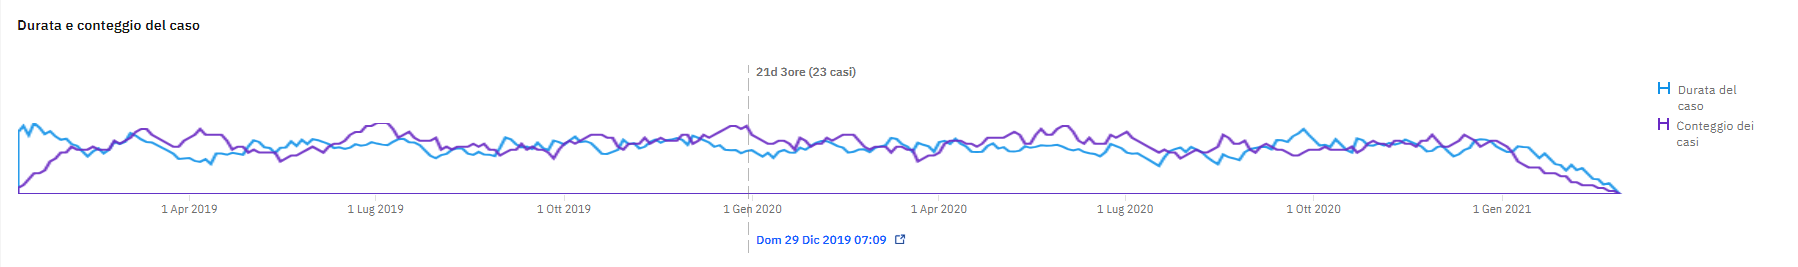
\includegraphics[width=\textwidth]{imgIBM/Simulazione/DurataConteggiSimulazione.png}
    \caption{Grafico della durata e conteggio dei casi}
    \label{fig:chart-duration-case-count}
\end{figure}
Il grafico serve come uno strumento di monitoraggio e analisi delle prestazioni del processo nel tempo. La possibilità di visualizzare sia il conteggio dei casi che la durata del caso in modo simultaneo è un punto chiave, poiché permette agli utenti di individuare correlazioni tra questi due parametri.\\
\begin{itemize}
    \item \custombold{Durata del caso} (linea azzurra): rappresenta quanto tempo è necessario, in media, per completare un singolo caso;
    \item \custombold{conteggi dei casi} (linea viola): mostra la quantità di casi trattati in un determinato periodo.
\end{itemize}
Dal punto di vista funzionale, questo tipo di grafico offre numerosi vantaggi. In particolare, fornisce una visione d'insieme dinamica e facilmente comprensibile per gli analisti di processo. L'andamento temporale consente di vedere con facilità trend a lungo termine, oltre a isolare specifici periodi in cui si verificano variazioni rilevanti.\\
Un altro punto di forza è la rappresentazione simultanea delle due metriche. Ciò consente di esaminare visivamente se gli aumenti nella durata del caso sono correlati a un aumento del numero di casi gestiti o se esistono periodi in cui si presentano disallineamenti tra i due parametri. Questa funzionalità è particolarmente utile per l'ottimizzazione del processo, poiché consente agli utenti di individuare non solo problemi di capacità, ma anche opportunità per migliorare l'efficienza, soprattutto quando si osservano periodi in cui la durata aumenta anche senza un corrispondente incremento dei volumi.

\subsubsection{Panoramica attività}
 \begin{figure}[H]
    \centering
    \includegraphics[width=\textwidth]{imgIBM/Simulazione/PanoramicaAttivitàSimulazione.png}
    \caption{Grafici della panoramica delle attività}
    \label{fig:activity-overview-graphs}
\end{figure}
La funzione di "Panoramica attività" permette di avere una visione globale dell'andamento di una specifica attività, come può essere l'inizio di un ciclo di produzione, all'interno di un processo complesso. L'obiettivo principale è quello di consentire agli analisti di comprendere come le attività si comportano nel tempo e se emergono criticità legate ai tempi di esecuzione o ai colli di bottiglia.\\
Offrendo informazioni sia sul conteggio delle attività che sui tempi di attesa e durata, questa funzionalità consente di analizzare non solo il volume delle attività, ma anche la loro efficienza operativa e la capacità del sistema di gestire il carico di lavoro senza subire rallentamenti.\\
I dati sono presentati in due grafici distinti, con metriche ben separate: il primo grafico mostra l'andamento della durata dell'attività e il conteggio delle attività eseguite, mentre il secondo si concentra sulla coda di attesa delle attività stesse. Questa separazione facilita la comprensione delle due dinamiche chiave: il volume di attività gestito e l'eventuale sovraccarico dovuto a tempi di attesa elevati.\\
La sovrapposizione di più metriche su uno stesso grafico permette inoltre una visione simultanea di come i volumi operativi influiscano sui tempi di completamento. Questo aiuta a visualizzare le relazioni tra gli elementi, ad esempio identificando se un aumento del numero di attività coincide con un allungamento dei tempi di attesa o se ci sono altre correlazioni significative.\\
Un altro vantaggio significativo di questa funzionalità è la possibilità di personalizzare la visualizzazione. Gli utenti possono selezionare l’attività specifica di interesse, come nel caso dell'“Inizio ciclo di produzione” mostrato nell'immagine, e concentrarsi su quella fase specifica del processo. Questo permette di affinare l'analisi, adattandola alle esigenze aziendali o a determinate unità operative, fornendo così informazioni più contestuali e rilevanti.\\

\subsection{Analytics}
La funzionalità "Analytics" nello strumento di process mining di IBM permette agli utenti di creare dashboard personalizzate e basate sui dati forniti dal sistema. Questo strumento consente una comprensione approfondita delle prestazioni operative, offrendo una visione chiara di come i processi si comportano nel tempo e fornendo strumenti visivi per analizzare i dati in modo semplice ed efficace.\\
Gli utenti possono personalizzare i propri pannelli di controllo utilizzando grafici, tabelle e KPI che riflettono le priorità aziendali e le performance chiave.\\
Una parte centrale di "Analytics" è la possibilità di analizzare le varianti del processo, una funzione che consente di vedere le deviazioni rispetto ai flussi di lavoro standard e di identificare quali di queste portano a migliori risultati o a inefficienze.\\
\end{document}